\documentclass[a4paper]{article}
\usepackage[english]{babel}
\usepackage[utf8]{inputenc}
\usepackage{fancyhdr}
\usepackage{hyperref}
\usepackage{amsmath,amsfonts,amssymb,amsthm}
\usepackage[a4paper, bottom=1.3in, top=1.3in, right=1in, left=1in]{geometry}
\usepackage[usenames,dvipsnames]{xcolor}
\usepackage[lined,boxed]{algorithm2e}
\usepackage{natbib}
\usepackage{tikz}
\usepackage{wrapfig}
\usetikzlibrary{calc}
\definecolor{amaranth}{rgb}{0.9, 0.17, 0.31}
\newcommand{\rcol}[1]{{\color{amaranth}#1}}

\newcommand{\wh}[1]{\widehat{#1}}
\newcommand{\wt}[1]{\widetilde{#1}}
\newcommand{\transp}{\intercal}

%%%%%%%%%%%%%%%%%%%%%%%%%%%%%%%%%%%%%%%%%%%
% Insert your name here
\newcommand{\fullname}{FILL fullname command at the beginning of latex document}
%%%%%%%%%%%%%%%%%%%%%%%%%%%%%%%%%%%%%%%%%%%

\newcommand{\lecture}[3]{
   \pagestyle{myheadings}
   \thispagestyle{plain}
   \newpage
   \setcounter{page}{1}
   \noindent
   \begin{center}
   \framebox{
      \vbox{\vspace{2mm}
              \hbox to .97\textwidth { {\bf MVA: Reinforcement Learning (2020/2021) \hfill Homework 2} }
       \vspace{6mm}
       \hbox to .97\textwidth { {\Large \hfill #1 \hfill } }
       \vspace{6mm}
       \hbox to .97\textwidth { {Lecturers: \it A. Lazaric, M. Pirotta  \hfill {{\footnotesize(\today)}}} }
      \vspace{2mm}}
   }
   \end{center}
   Solution by {\color{amaranth}\fullname}
   \markboth{#1}{#1}
   \vspace*{4mm}
}


\DeclareMathOperator*{\argmax}{\arg\,\max}
\DeclareMathOperator*{\argmin}{\arg\,\min}
\DeclareMathOperator*{\arginf}{\arg\,\inf}


\setlength{\parindent}{0cm}
\begin{document}
\lecture{Approximate Reinforcement Learning}{1}


\pagestyle{fancy}
\fancyhf{}
\rhead{Full name: {\color{amaranth}\fullname}}
\lhead{(Approximate) Reinforcement Learning}
\cfoot{\thepage}

\textbf{Instructions}
\begin{itemize}
    \item The deadline is \textbf{December 21, 2020. 23h00}
    \item By doing this homework you agree to the \emph{late day policy, collaboration and misconduct rules} reported on \href{https://piazza.com/class/kf86owfvi2u2lg?cid=8}{Piazza}.
    \item \textbf{Mysterious or unsupported answers will not receive full credit}.
    A correct answer, unsupported by calculations, explanation, or algebraic work will receive no credit; an incorrect answer supported by substantially correct calculations and explanations might still receive partial credit.
    \item Answers should be provided in \textbf{English}.
\end{itemize}


\section{TRPO}
Compare Conservative Policy Iteration (\url{https://people.eecs.berkeley.edu/~pabbeel/cs287-fa09/readings/KakadeLangford-icml2002.pdf}) and TRPO (\url{https://arxiv.org/abs/1502.05477}). Highlight similarities and differences.

\section{Linear TD}
Consider the Linear TD(0) algorithm. Given a tuple $(s_t, a_t, s_{t+1}, r_t)$ such that $s_{t+1} \sim p(\cdot| s_t,a_t)$ with $a_t \sim  \pi$ and $r_t \sim r(s_t, a_t)$, the TD update rule is given by
\begin{align*}
    \theta_{t+1} = \theta_t + \alpha \Big(r_t + \gamma \phi_{t+1}^\transp \theta_t - \phi_t^\transp \theta_t\Big) \phi_t
\end{align*}
where $\phi_t = \phi(s_t)$ and $\alpha_t \geq  0$.
We ask to characterize the expected behavior of the steps taken by the TD algorithm in ``steady state''.
Let $A = \mathbb{E}[\phi_t(\phi_t  - \gamma \phi_{t+1})]$ and $b = \mathbb{E}[r_t \phi_t]$ be the steady state matrices, where the expectation is such that $s_t \sim d^{\pi}$, $s_{t+1} \sim p(\cdot| s_t, a_t)$,  $a_t \sim \pi(\cdot|s_t)$. Note that $d^{\pi}$ is the stationary distribution of policy $\pi$.
\begin{enumerate}
    \item Write the expected updated $\mathbb{E}[\theta_{t+1}| \theta_t]$ as a function of  $A$ and $b$. If the process converges, what is the fixed point?
    \item If correctly derive, you should notice that $A$ plays a central role in the stability of the update. If  $A$ is positive definite, $\theta_t$ shrinks at every update. Given the definition of $A$ show that $A = \Phi^\transp D (I - \gamma P) \Phi$ for appropriate matrices.
    \item Given this decomposition show that $A$ is positive definite.\\
    Hints: 1) Any matrix $M$ is positive definite if and only if the symmetric matrix $S = M + M^\transp$ is positive definite. 
    2) Any symmetric real matrix $S$ is positive definite if all of its diagonal entries are positive and greater
    than the sum of the absolute values of the corresponding off-diagonal entries.
\end{enumerate}
This shows that the TD(0) update is stable in the stationary regime. Additional conditions and steps are necessary to prove convergence.


\paragraph{Off-policy learning.}
Often we have access to a large amount of data collected through a set of different policies, called behavioral policies.
The objective will be to use these samples to compute the value function of a target policy $\pi$. For simplicity suppose that we have a single behavioral policy $\rho \neq \pi$. 
The off-policy Linear TD(0)~\citep{PrecupSD01} is simply
\begin{align}\label{eq:offtdlin}
    \theta_{t+1} = \theta_t + \alpha \boldsymbol{w_t} \Big(r_t + \gamma \phi_{t+1}^\transp \theta - \phi_t^\transp \theta_t\Big) \phi_t
\end{align}
where $w_t = \frac{\pi(a_t|s_t)}{\rho(a_t|s_t)}$ is the importance weight.

\begin{itemize}
    \item Consider the following MDP with $2$ states and $2$ actions
    \begin{center}
        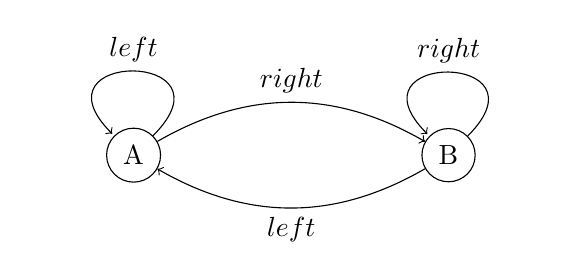
\begin{tikzpicture}
            \node[circle, draw] (A) at (0,0) {A};
            \node[circle, draw] (B) at (4,0) {B};
            \path[->] (A) edge[bend left] node[above] {$right$} (B);
            \path[->] (B) edge[bend left] node[below] {$left$} (A);
            \path[->] (B) edge[loop] node[above] {$right$} (B);
            \path[->] (A) edge[loop] node[above] {$left$} (B);
        \end{tikzpicture}
    \end{center}
    Consider a behavioral policy $\rho(right| \cdot) = 1/2$ and a target policy $\pi(right|\cdot) = 1$. 
    The reward function is $0$ everywhere and the value function is parametrized through a single parameter $\theta$ such that $V(A)= 0.8\theta$ and $V(B) = 2\theta$.
    Show that the update~\eqref{eq:offtdlin} diverges. Assume that $\theta_t = 10$, $\alpha = 0.1$ and $\gamma =0.9$.
\end{itemize}

\section{REINFORCE}
In class we have seen the derivation of the policy gradient theorem in the ``Monte-Carlo style''. Recall that the policy gradient is given by
\[
    \nabla_\theta J(\pi_\theta) = \mathbb{E}_{\tau \sim \mathbb{P}(\cdot|\pi_\theta)}\left[ \nabla_\theta \log \mathbb{P}(\tau|\pi_\theta) 
    R(\tau)
    \right]
\]
where $R(\tau) = \sum_{t=1}^{|\tau|} r_t$. % and $b(\tau)$ is a baseline.

\begin{itemize}
    \item By construction the policy gradient is on-policy. Derive an off-policy variant by assuming to collect samples from a behavioral policy $\mu(s,a)$. The target policy, i.e., the policy for which we want to compute the gradient is $\pi_{\theta}$
\end{itemize}

So far we have seen the ``Monte Carlo'' derivation of the gradient.
It is possible to derive the gradient theorem by leveraging the recursive structure of the Bellman equation. Recall that for a $\gamma$-discounted infinite-horizon MDP, we define the policy performance $J(\pi_\theta) = \mathbb{E}\left[\sum_{t=1}^{+\infty} \gamma^{t-1} r_t | s_1 \sim \rho, \pi_\theta \right]$. Then, the policy gradient is given by
\begin{align}
    \label{eq:pgt}
    \nabla_\theta J(\theta) = \mathbb{E}_{s \sim d^{\pi_\theta}} \mathbb{E}_{a \sim \pi_\theta(s, \cdot)}
    \left[ 
        \nabla_{\theta} \log \pi_\theta(s,a) Q^\pi(s,a)
    \right]
\end{align}
where $d^{\pi_\theta}(s) = \lim_{T \to \infty} \sum_{t=1}^{T} \gamma^{t-1} \mathbb{P}(s_t=s|\pi,s_1 \sim \rho)$.

\begin{itemize}
    \item Derive the gradient in Eq.~\ref{eq:pgt}. \emph{Hint: you can start from $V^{\pi}(s) = \sum_a \pi(s,a) Q^{\pi}(s,a)$}
\end{itemize}
\begin{wrapfigure}{r}{0.4\textwidth}
    \centering
    \includegraphics[width=.4\textwidth]{Untitled}
    \caption{DQN network (left) and partial Dueling DQN (right).}
    \label{fig:net}
    \vspace{-50pt}
\end{wrapfigure}

\section{DQN}
The goal of this exercise is to compare different variants of Deep Q-Learning (a.k.a. DQN).

\paragraph{DQN.} Recall from the class the DQN aims to minimize the following loss function
\[
    L(\theta) = \mathbb{E}_{s,a,r,s' \sim \mathcal{D}} \left[
\left(
    r + \gamma \max_{a' \in\mathcal{A}} Q(s',a';\theta') - Q(s,a; \theta)
\right)^2
    \right ]
\]
where $\theta'$ is the parameter of the target network updated every $C$ iterations from $\theta$.
\begin{enumerate}
    \item (written) This objective resembles a classical supervised learning problem. Could you highlight the differences?
    \item (written) Could you describe the role of $C$ and the trade-off at play in choosing a good value for $C$?
\end{enumerate}


\vspace{.2in}
\emph{Replay Memory.} As we play, we store our transitions $(s, a, r, s')$ in a buffer $\mathcal{D}$. Old examples are deleted as we store new transitions. To update our parameters, we sample a minibatch from the buffer and perform a stochastic gradient descent update.

\vspace{.2in}
\emph{$\epsilon$-greedy exploration.} For exploration, we use an $\epsilon$-greedy strategy. It is standard to use a linear annealing schedule from $\epsilon_{start}$ to $\epsilon_{\min}$.

\vspace{.2in}
\emph{Q-function representation.} As suggested in the original paper, the Q-function is represented using a neural network with input a state $s$ and output a vector of dimension $|\mathcal{A}|$ containing the estimated Q-value for each action $a \in \mathcal{A}$.
\begin{enumerate}
    \item (written) What is one benefit of representing the Q function as $Q(s; \theta) \in \mathbb{R}^{|\mathcal{A}|}$?
\end{enumerate}

Implementation
\begin{enumerate}
    \item (code) Implement DQN. We provided an almost complete version of DQN in \texttt{dqn\_start.py.py}.
    Implement the network on Fig.~\ref{fig:net}(left).
\end{enumerate}
The code generates two plots. The first plot shows the performance (cumulative reward) over the learning process (i.e., as a function of time steps). The second figure shows the performance of the associated greedy policy on a test environment averaged over multiple episodes.\footnote{Usually, this metric is evaluated less frequently since it is more computationally costly. It is a parameter in the code. By default we run every 2 episodes.} It also saves the results in a file called \texttt{dqn\_results.txt}.
\begin{enumerate}
    \item (code) A single run is not enough to evaluate the performance of an algorithm. To have significant results, we need to perform multiple repetitions. Change the code to run multiple versions of DQN and reports the average performance and uncertainty as function of time steps (for both figures). We provide a script that reads files generated by \texttt{dqn\_start.py.py} that can be used to generate the requested figures.\footnote{It is not necessary to use this script to generate figures.}
\end{enumerate}

\paragraph{Competitors.} We would like to evaluate DQN with newer variants of DQN, namely Double DQN and Dueling DQN.
In class we have seen the principle of Double DQN while we refer to the original paper for Dueling DQN (\url{https://arxiv.org/abs/1511.06581}).

The difference between DQN and Double DNQ is how the target network is built. In Double DQN we use the greedy action suggested by $Q(s,a; \boldsymbol{\theta})$ to evaluate the target (i.e., $\theta'$), see the appendix of \url{https://arxiv.org/abs/1511.06581}.
In Dueling DQN, the Q function is estimated as
\[
    Q(s,a) = V(s) + A(s,a) - \frac{1}{|\mathcal{A}|} \sum_{a'} A(s,a')
\]
$V$ and $A$ share parameters.
Dueling DQN can be implemented ``standard'' or ``double''.

Starting from the code of \texttt{dqn\_start.py.py},
\begin{enumerate}
    \item (code) Implement Double DQN. Use the same network of DQN.
    \item (code) Implement Dueling Double DQN. See Fig.~\ref{fig:net} for the network with shared parameters.
    \item Compare the performance of the algorithms
\end{enumerate}

\bibliographystyle{plainnat}
\bibliography{bibliography}
\end{document}